\documentclass[a4paper,12pt]{article}
\usepackage{float}
\usepackage{placeins}

\usepackage{ucs}
\usepackage[utf8x]{inputenc}
%\usepackage[latin1]{inputenc}
\usepackage[T1]{fontenc}

\usepackage[french]{babel}

\pagestyle{plain}

\usepackage{graphicx}
\usepackage{subfigure}
\DeclareGraphicsExtensions{.pdf,.eps,.jpg,.png,.gif}




%%%%%%%%%%%%%%%%%%%%%%%%%%%%%%%%%%%%%%%%%%%%%%%%%%%%%%%%%%%%

\author{
  Xavier \textsc{Fraboulet}, Paul \textsc{CHaignon} \\ \\
  INSA de Rennes \\
  4INFO, groupe 2.2
}

\title{Guide d'utilisateur \\ SmallWorld}

\begin{document}
\maketitle

\thispagestyle{empty}
\newpage

~~
\thispagestyle{empty}
\newpage


\tableofcontents
\newpage

\section{Bienvenue dans SmallWorld !}

Vous vous apprêtez à rentrer dans le monde de SmallWorld, un monde remplit de dangers et d'ennemis redoutables. Depuis la nuit des temps, les terribles Vikings, les vaillants Gaulois et les hargneux Nains s'opposent pour le contrôle de ce monde. 

SmallWorld est un jeu tour-par-tour où le but est de gérer des unités sur une carte afin d'obtenir le plus de points possible à l'issue de la partie. Plus le joueur contrôle de cases de la carte plus il gagne de points. De plus, il est possible d'attaquer les unités du joueur adverse afin de contrôler plus de cases. Dans ce jeu, deux joueurs s'opposeront et pourront jouer trois peuples différents : les nains, les gaulois ou les vikings.



\section{La carte}
La carte du monde se compose de cases carrées. Il existe différents types de case : montagne, plaine, désert, eau, forêt. La carte est créée de manière aléatoire.

Il existe 3 types de cartes :

\begin{itemize}
\item Démo : 2 joueurs, 5 cases × 5 cases, 5 tours, 4 unités par peuples ;
\item Petite : 2 joueurs, 10 cases × 10 cases, 20 tours, 6 unités par peuples ;
\item Normale : 2 joueurs, 15 cases × 15 cases, 30 tours, 8 unités par peuples.
\end{itemize}


\section{Les peuples et unités}
À chaque tour, toutes les unités peuvent se déplacer ou attaquer. Par défaut (c.-à-d. hors bonus), chaque unité peut se déplacer d’une case par tour. Chaque unité possède 5 d’attaque, 2 de défense et 5 points de vie. Aussi par défaut, elle rapporte un point à chaque tour.

\subsection{Gaulois}
Le coût de déplacement sur une case de plaine est divisé par deux.

Une unité gauloise fournit un point de plus lorsqu'elle occupe une case de type plaine.

Une unité gauloise n'acquière aucun point sur les cases de type montagne.

\subsection{Vikings}
Une unité Viking a la capacité de se déplacer sur l’eau. L’occupation d’une case eau ne
rapporte cependant aucun point.

Une unité Viking fournit 1 point de plus lorsqu’elle occupe une case au bord de l’eau.

Une unité Viking n’acquière aucun point sur les cases de type désert.

\subsection{Nains}
Lorsqu’elle se trouve sur une case montagne, une unité Nain a la capacité de se déplacer
sur n’importe quelle case montage de la carte à condition qu’elle ne soit pas occupée par
une unité adverse.

Une unité Nain fournit 1 point de plus lorsqu’elle occupe une case forêt.

Une unité Nain n’acquière aucun point sur les cases de type plaine.

\section{Gestion des parties}
\subsection{Création d'une nouvelle partie}
Lorsque vous cliquez sur l'exécutable, une fenêtre apparait (fig \ref{fig:create}) et vous permet de créer une nouvelle partie. Remplissez les champs et cliquez sur "Launch" pour lancer la partie.

\begin{figure}[H]
   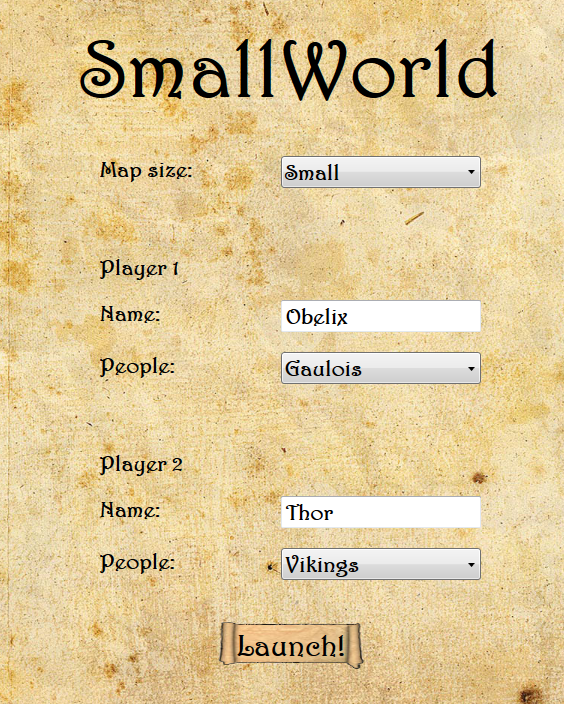
\includegraphics[width=\textwidth]{create.png}
   \label{fig:create}
   \caption{Fenêtre de création d'une partie.}
\end{figure}
\FloatBarrier

\subsection{Chargement d'une partie enregistrée}
Dans le menu, sélectionnez "open" puis naviguez jusqu'au dossier contenant le fichier de jeu. Celui a pour extension ".sav".

\subsection{Sauvegarde d'une partie}
Pour sauvegarder une partie, vous devez aller dans le menu et sélectionner "save as" si vous sauvegardez pour la première fois ou "save" si la partie a déjà été sauvegardée une première fois.


\section{Déroulement du jeu}
\begin{figure}[H]
   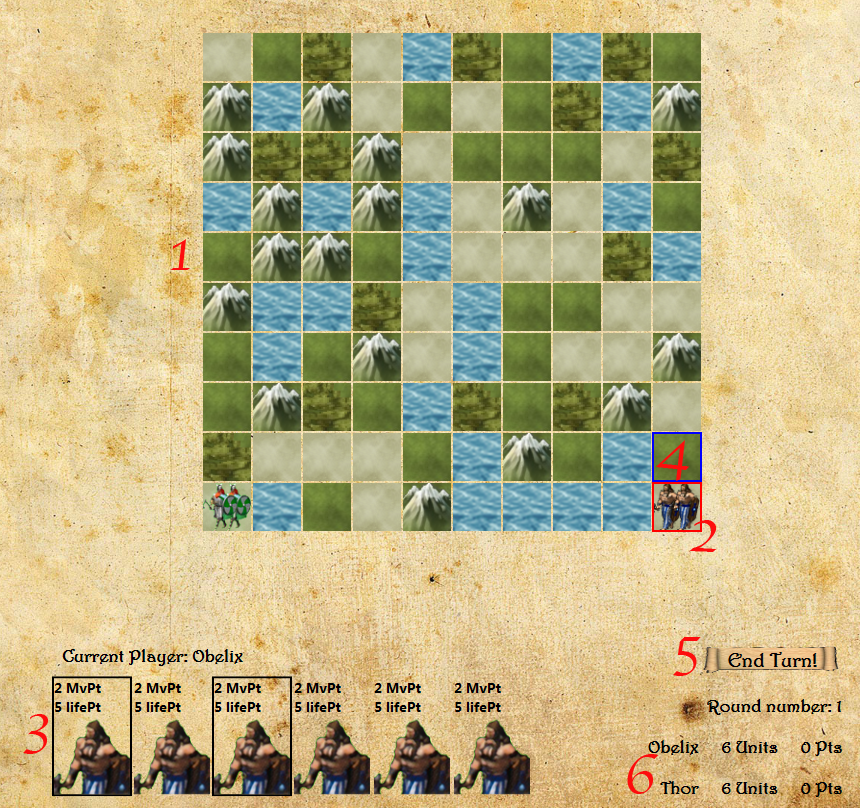
\includegraphics[width=\textwidth]{game.png}
   \label{fig:create}
   \caption{Fenêtre du jeu.}
\end{figure}
\FloatBarrier

\begin{enumerate}
\item la carte ;
\item la case sélectionnée ;
\item le sélectionneur d'unités ;
\item les cases suggérées ;
\item le bouton pour mettre fin au tour ;
\item les informations sur la partie (nombre de points et unités pour les joueurs).
\end{enumerate}


\subsection{Déroulement d'un tour}
\subsubsection{Déplacement d'une unité}
Lors d'un tour, vous allez être amené à déplacer des unités. Pour ce faire, vous devez :
\begin{itemize}
\item \textbf{Sélectionner une case en utilisant le clique gauche de la souris}. Si la case contient des unités de votre peuple, elles s'afficheront en bas à gauche de l'écran dans le "sélecteur d'unités" ;
\item Par défaut, une unité est sélectionnée dans le sélecteur, mais vous pouvez en choisir une autre en cliquant avec le bouton gauche de la souris. Une fois sélectionnée, l'unité est entourée en noir ;
\item Lorsqu'une unité est sélectionnée, vous pouvez la \textbf{déplacer sur la carte en utilisant le bouton droit de la souris} ;
\item Si la case est occupée par des unités adverses, un combat commencera.
\end{itemize}

\subsubsection{Sélection multiple d'unités}
Il est possible de sélectionner plusieurs unités en même temps. Pour ce faire, vous pouvez :
\begin{itemize}
\item Maintenir la touche "Ctrl" et cliquer sur une case de la carte : toutes les unités de la case seront sélectionnées.
\item Maintenir "Ctrl" et cliquer sur les différentes unités du "sélecteur d'unités" afin de sélectionner les unités une par une.
\end{itemize}

\subsubsection{Suggestion de cases}
Lorsque vous sélectionnez une unité, des suggestions de cases apparaissent en bleu sur la carte.

\subsection{Fin d'un tour}
Pour mettre fin à un tour, deux options s'offrent à vous :
\begin{itemize}
\item Fin du tour en cliquant sur le bouton "End Round!" ;
\item Fin automatique du tour lorsque toutes les unités n'ont plus de points de déplacement.
\end{itemize}

\subsection{Fin du jeu}
À la fin de chaque tour, le jeu vérifie si un des joueurs à gagner, plusieurs scénarios existent :
\begin{itemize}
\item Un joueur n'a plus d'unité, l'autre joueur gagne la partie ;
\item À l'issu du nombre de tour défini par le type de la carte, le joueur ayant le plus de points remporte la partie.
\end{itemize}


\end{document}
